% !TeX program = xelatex
% The three primary report identity fields can be edited here.
\newcommand{\reporttitle}{Model Training and Results for the bir.mov Recommender System}
\newcommand{\reportauthor}{bir.mov Project}
\newcommand{\reportdate}{July 17, 2026}

\documentclass[11pt,a4paper]{article}

\usepackage[a4paper,top=22mm,bottom=24mm,left=23mm,right=23mm,headheight=22pt]{geometry}
\usepackage{fontspec}
\IfFontExistsTF{TeX Gyre Pagella}{
  \setmainfont{TeX Gyre Pagella}
  \setsansfont{TeX Gyre Heros}
  \setmonofont{TeX Gyre Cursor}[Scale=0.82]
}{
  % Fallback for sandboxed macOS environments where fontconfig cannot write its cache.
  \newcommand{\texgyredir}{/usr/local/texlive/2025/texmf-dist/fonts/opentype/public/tex-gyre/}
  \setmainfont[
    Path=\texgyredir,
    UprightFont=texgyrepagella-regular.otf,
    BoldFont=texgyrepagella-bold.otf,
    ItalicFont=texgyrepagella-italic.otf,
    BoldItalicFont=texgyrepagella-bolditalic.otf
  ]{TeX Gyre Pagella}
  \setsansfont[
    Path=\texgyredir,
    UprightFont=texgyreheros-regular.otf,
    BoldFont=texgyreheros-bold.otf,
    ItalicFont=texgyreheros-italic.otf,
    BoldItalicFont=texgyreheros-bolditalic.otf
  ]{TeX Gyre Heros}
  \setmonofont[
    Path=\texgyredir,
    Scale=0.82,
    UprightFont=texgyrecursor-regular.otf,
    BoldFont=texgyrecursor-bold.otf,
    ItalicFont=texgyrecursor-italic.otf,
    BoldItalicFont=texgyrecursor-bolditalic.otf
  ]{TeX Gyre Cursor}
}
\usepackage{microtype}
\usepackage{graphicx}
\graphicspath{{../../docs/}}
\usepackage{booktabs}
\usepackage{tabularx}
\usepackage{array}
\usepackage{multirow}
\usepackage{enumitem}
\usepackage{amsmath,amssymb}
\usepackage{xcolor}
\usepackage{tikz}
\usetikzlibrary{arrows.meta,backgrounds,calc,fit,positioning,shapes.geometric}
\usepackage{pgfplots}
\pgfplotsset{compat=1.18}
\usepackage{caption}
\usepackage{subcaption}
\usepackage{titlesec}
\usepackage{fancyhdr}
\usepackage{csquotes}
\usepackage{xurl}
\usepackage{hyperref}
\usepackage{float}

\definecolor{Ink}{HTML}{17202A}
\definecolor{Slate}{HTML}{53606D}
\definecolor{Rule}{HTML}{D9DEE5}
\definecolor{Blue}{HTML}{3B73D1}
\definecolor{Gold}{HTML}{D99A16}
\definecolor{Red}{HTML}{C54B45}
\definecolor{Green}{HTML}{3A8D6D}
\definecolor{Paper}{HTML}{F5F7FA}

\hypersetup{
  hypertexnames=false,
  colorlinks=true,
  linkcolor=Blue,
  citecolor=Green,
  urlcolor=Blue,
  pdftitle={\reporttitle},
  pdfauthor={\reportauthor}
}

\titleformat{\section}
  {\Large\bfseries\sffamily\color{Ink}}
  {\thesection}{0.65em}{}
  [\vspace{0.25em}\color{Rule}\titlerule]
\titleformat{\subsection}
  {\large\bfseries\sffamily\color{Ink}}
  {\thesubsection}{0.55em}{}
\titleformat{\subsubsection}
  {\normalsize\bfseries\sffamily\color{Ink}}
  {\thesubsubsection}{0.5em}{}
\titlespacing*{\section}{0pt}{2.3ex plus 0.5ex}{1.2ex}
\titlespacing*{\subsection}{0pt}{1.8ex plus 0.4ex}{0.8ex}

\pagestyle{fancy}
\fancyhf{}
\fancyhead[L]{\sffamily\small bir.mov - Model Training Report}
\fancyhead[R]{\sffamily\small \reportdate}
\fancyfoot[C]{\sffamily\small\thepage}
\renewcommand{\headrulewidth}{0.4pt}
\renewcommand{\headrule}{\hbox to\headwidth{\color{Rule}\leaders\hrule height \headrulewidth\hfill}}

\captionsetup{font=small,labelfont={bf,sf},textfont=it,justification=centering}
\setlist[itemize]{leftmargin=1.5em,itemsep=0.25em,topsep=0.35em}
\setlist[enumerate]{leftmargin=1.7em,itemsep=0.25em,topsep=0.35em}
\renewcommand{\arraystretch}{1.18}
\emergencystretch=3em
\newcolumntype{Y}{>{\raggedright\arraybackslash}X}
\newcolumntype{C}[1]{>{\centering\arraybackslash}p{#1}}
\newcommand{\metric}[1]{\textbf{\sffamily\color{Ink}#1}}
\newcommand{\file}[1]{\nolinkurl{#1}}
\newcommand{\sourceNote}[1]{\par\vspace{0.35em}{\footnotesize\color{Slate}\textit{Source: #1}\par}}

\newenvironment{keybox}
{\begin{center}\begin{minipage}{0.93\textwidth}\color{Ink}\hrule\vspace{0.7em}}
{\vspace{0.7em}\hrule\end{minipage}\end{center}}

\begin{document}

% -----------------------------------------------------------------------------
% Cover
% -----------------------------------------------------------------------------
\begin{titlepage}
\thispagestyle{empty}

\begin{tikzpicture}[remember picture,overlay]
  \fill[Ink] (current page.north west) rectangle ($(current page.south east)+(0,95mm)$);
  \fill[Gold] ($(current page.north west)+(0,-95mm)$) rectangle ($(current page.north east)+(0,-98mm)$);
  \fill[Paper] ($(current page.south west)+(0,0)$) rectangle ($(current page.south east)+(0,95mm)$);
  \node[anchor=north west,text=white,font=\sffamily\bfseries\fontsize{31}{34}\selectfont]
    at ($(current page.north west)+(23mm,-24mm)$) {bir\textcolor{Red}{\textperiodcentered}mov};
  \node[anchor=north west,text width=160mm,text=white,font=\sffamily\bfseries\fontsize{24}{29}\selectfont]
    at ($(current page.north west)+(23mm,-51mm)$) {Model Training and Results\\for the Recommender System};
  \node[anchor=north west,text width=155mm,text=white!78,font=\sffamily\fontsize{11.5}{16}\selectfont]
    at ($(current page.north west)+(23mm,-115mm)$)
    {A technical review of the explicit-feedback MF and implicit-feedback ALS models trained on MovieLens ml-32m, covering methodology, experimental design, quantitative results, and production use};
  \node[anchor=north west,text width=160mm,text=Ink,font=\sffamily\fontsize{11}{16}\selectfont]
    at ($(current page.south west)+(23mm,70mm)$)
    {\textbf{Prepared by}\quad \reportauthor\\[2mm]
     \textbf{Report date}\quad \reportdate\\[2mm]
     \textbf{Models reviewed}\quad \file{ml32m-mf128-v1} and \file{ml32m-als128-v1}};
  \node[anchor=south west,text width=160mm,text=Slate,font=\sffamily\fontsize{9}{12}\selectfont]
    at ($(current page.south west)+(23mm,18mm)$)
    {The experimental values in this report were verified against saved notebook outputs and model metadata. The training pipeline was not rerun while preparing this document.};
\end{tikzpicture}
\end{titlepage}

\pagenumbering{roman}
\tableofcontents
\clearpage

\section*{Executive Summary}
\addcontentsline{toc}{section}{Executive Summary}

bir.mov uses a hybrid recommendation architecture that assigns two distinct tasks to two specialized models. \textbf{ALS-128} ranks unseen candidate films from the user's positive history. \textbf{MF-128} predicts the 0.5-5.0 star rating that the user is likely to assign to each candidate. The offline results directly support this separation of responsibilities.

\begin{keybox}
\begin{tabularx}{\textwidth}{@{}Y C{29mm} C{48mm}@{}}
\toprule
\textbf{Key finding} & \textbf{Result} & \textbf{Interpretation} \\
\midrule
MF rating prediction & Test RMSE: \metric{0.8244} & \metric{5.9\%} lower than the bias baseline \\
ALS Top-10 ranking & Recall@10: \metric{0.0842} & \metric{72.2\%} above the popularity baseline \\
ALS Top-10 ranking & NDCG@10: \metric{0.0668} & \metric{55.3\%} above the popularity baseline \\
MF Top-10 ranking & Recall@10: \metric{0.0005} & Accurate ratings, but unsuitable for direct catalog ranking \\
\bottomrule
\end{tabularx}
\end{keybox}

The central result is the alignment between optimization objective and production role. Explicit-feedback MF minimizes star-rating error, while implicit-feedback ALS is optimized to retrieve liked films near the top of the list. The production implementation follows this evidence: ALS generates a broad candidate pool, MF assigns personalized rating estimates, and a final layer combines genre preference, IMDb quality, similarity to liked and disliked films, novelty, and list diversity.

One limitation is essential to the interpretation of this report. The offline experiment evaluates the base MF and ALS models. The notebook does not contain a separate end-to-end test of the production hybrid reranker. The report therefore does not claim a measured numerical gain for that final layer.

\clearpage
\pagenumbering{arabic}

% -----------------------------------------------------------------------------
\section{Project Objective and Model Architecture}

bir.mov generates personalized movie recommendations by matching ratings exported from IMDb or Letterboxd to the MovieLens catalog. The system answers two different questions with two different models:

\begin{enumerate}
  \item \textbf{Which films should rank highest?} Implicit-feedback ALS produces a candidate ranking from the user's positive history.
  \item \textbf{What rating will the user give this film?} Explicit-feedback MF predicts a personal score on the star-rating scale.
\end{enumerate}

\begin{figure}[H]
\centering
\resizebox{\textwidth}{!}{%
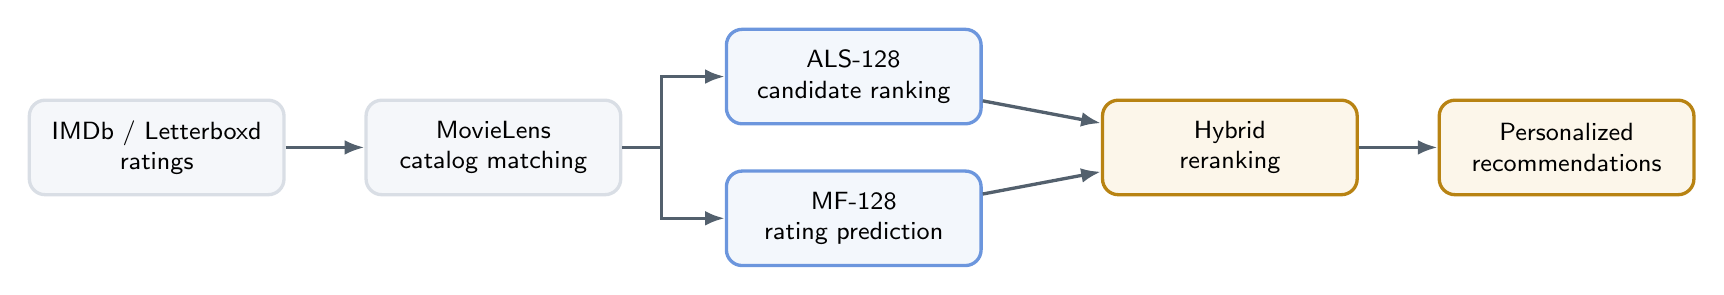
\begin{tikzpicture}[
  node distance=8mm and 10mm,
  box/.style={rounded corners=2mm,draw=Rule,very thick,fill=Paper,minimum height=12mm,text width=30mm,align=center,font=\sffamily\small},
  model/.style={box,draw=Blue!75,fill=Blue!6},
  resultbox/.style={box,draw=Gold!85!black,fill=Gold!9},
  arrow/.style={-{Latex[length=2.5mm]},very thick,draw=Slate}
]
  \node[box] (upload) {IMDb / Letterboxd\\ratings};
  \node[box,right=of upload] (match) {MovieLens\\catalog matching};
  \node[model,right=13mm of match,yshift=9mm] (als) {ALS-128\\candidate ranking};
  \node[model,right=13mm of match,yshift=-9mm] (mf) {MF-128\\rating prediction};
  \node[resultbox,right=15mm of als,yshift=-9mm] (rerank) {Hybrid\\reranking};
  \node[resultbox,right=of rerank] (result) {Personalized\\recommendations};
  \draw[arrow] (upload) -- (match);
  \draw[arrow] (match.east) -- ++(5mm,0) |- (als.west);
  \draw[arrow] (match.east) -- ++(5mm,0) |- (mf.west);
  \draw[arrow] (als) -- (rerank);
  \draw[arrow] (mf) -- (rerank);
  \draw[arrow] (rerank) -- (result);
\end{tikzpicture}}
\caption{Separation of responsibilities between the two production models.}
\label{fig:architecture}
\end{figure}

This architecture is designed for new-user inference. A person uploading ratings is not represented in the original MovieLens user vocabulary. At request time, the system recomputes the person's representation against fixed movie factors. Section~\ref{sec:serving} describes this \textit{fold-in} process in detail.

% -----------------------------------------------------------------------------
\section{Dataset and Preprocessing}

\subsection{MovieLens ml-32m overview}

The training source is MovieLens ml-32m \cite{harper2015movielens}. Table~\ref{tab:dataset} summarizes the raw tables recorded in the training notebook.

\begin{table}[H]
\centering
\caption{Key properties of the raw dataset.}
\label{tab:dataset}
\begin{tabularx}{0.84\textwidth}{@{}Y r@{}}
\toprule
\textbf{Property} & \textbf{Value} \\
\midrule
Users & 200,948 \\
Rated films & 84,432 \\
Catalog size in \file{movies.csv} & 87,585 \\
Ratings & 32,000,204 \\
Tag applications & 2,000,072 \\
Mean ratings per user & 159.2 \\
Rating mean / median / standard deviation & 3.540 / 3.5 / 1.059 \\
Rating time span & 1995-2023 \\
User-item matrix sparsity & 99.8114\% \\
\bottomrule
\end{tabularx}
\sourceNote{Recorded outputs in Section 1 of \file{train/ml-32m-train.ipynb}.}
\end{table}

The data exhibits a pronounced long tail. The median film has only 5 ratings, while the most popular film has 102,929. The top 1\% of films account for 54.8\% of all ratings. This structure makes poorly supported movie factors unstable and helps explain the extreme predictions observed when MF is used as a direct full-catalog ranker.

\subsection{Rare-film filtering and indexing}

Films with fewer than 5 ratings were removed from the model vocabulary. The filter discards 48.0\% of rated films while retaining 99.75\% of all rating events. The resulting model matrix contains 200,948 users and 43,884 films.

\begin{figure}[H]
\centering
\begin{subfigure}[t]{0.47\textwidth}
\centering
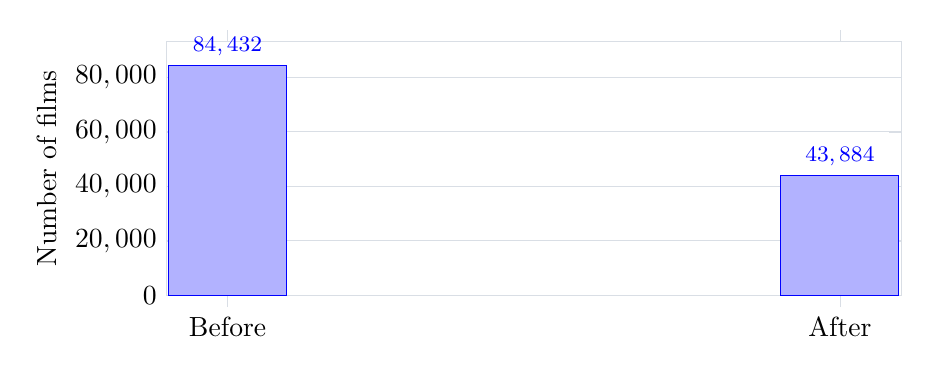
\begin{tikzpicture}
\begin{axis}[
  ybar, width=0.90\linewidth, height=48mm,
  symbolic x coords={Before,After}, xtick=data,
  ylabel={Number of films}, ymin=0, ymax=93000, scaled y ticks=false,
  yticklabel style={/pgf/number format/fixed,/pgf/number format/1000 sep={,}},
  bar width=15mm, nodes near coords,
  nodes near coords style={font=\footnotesize,/pgf/number format/1000 sep={,}},
  axis line style={draw=Rule}, tick style={draw=Rule},
  ymajorgrids, grid style={draw=Rule},
  every axis plot/.append style={fill=Blue,draw=Blue}
]
\addplot coordinates {(Before,84432) (After,43884)};
\end{axis}
\end{tikzpicture}
\caption{Change in the film vocabulary.}
\end{subfigure}
\hfill
\begin{subfigure}[t]{0.47\textwidth}
\centering
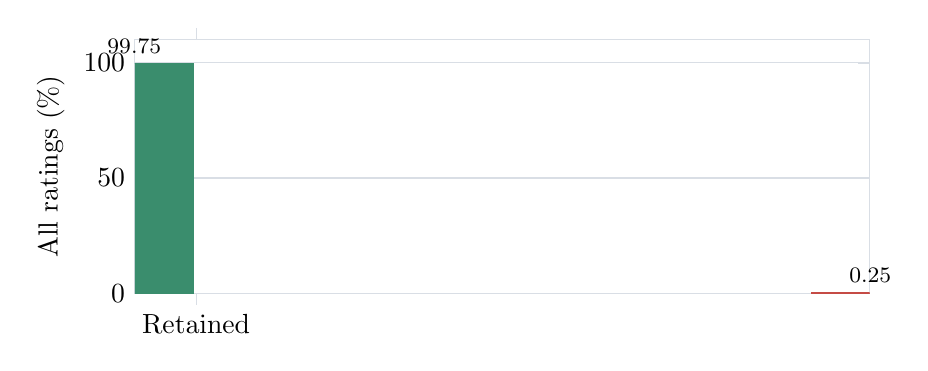
\begin{tikzpicture}
\begin{axis}[
  ybar, width=0.90\linewidth, height=48mm,
  symbolic x coords={Retained,Removed}, xtick=data,
  ylabel={All ratings (\%)}, ymin=0, ymax=110,
  bar width=15mm, nodes near coords,
  nodes near coords style={font=\footnotesize},
  axis line style={draw=Rule}, tick style={draw=Rule},
  ymajorgrids, grid style={draw=Rule}
]
\addplot[fill=Green,draw=Green] coordinates {(Retained,99.75)};
\addplot[fill=Red,draw=Red] coordinates {(Removed,0.25)};
\end{axis}
\end{tikzpicture}
\caption{Share of rating events retained.}
\end{subfigure}
\caption{Effect of the minimum-5-ratings filter.}
\label{fig:filter}
\end{figure}

MovieLens identifiers were converted to contiguous zero-based indices required by sparse matrices and embedding layers. The \file{user_ids.npy} and \file{movie_ids.npy} files preserve the mapping back to the original MovieLens identifiers.

\subsection{Per-user chronological split}

Ratings were sorted by timestamp within each user. The first 80\% were assigned to training, the next 10\% to validation, and the remainder to testing. A per-user chronological split uses the past to predict the future and reduces the future-information leakage associated with random splitting.

\begin{table}[H]
\centering
\caption{Chronological split after filtering.}
\label{tab:split}
\begin{tabular}{@{}lrr@{}}
\toprule
\textbf{Split} & \textbf{Ratings} & \textbf{Share} \\
\midrule
Training & 25,614,481 & 80.24\% \\
Validation & 3,200,365 & 10.03\% \\
Test & 3,106,621 & 9.73\% \\
\bottomrule
\end{tabular}
\end{table}

The training CSR matrix has a density of only 0.2905\%. This level of sparsity motivates low-dimensional latent-factor models and the sparse linear-algebra advantages of ALS.

% -----------------------------------------------------------------------------
\section{Evaluation Protocol}

The models optimize different objectives, so two metric families were used.

\subsection{Rating-prediction metrics}

MF and the rating baselines were evaluated from the error between the observed rating $r_{ui}$ and the estimate $\hat r_{ui}$:

\begin{align}
\mathrm{RMSE} &= \sqrt{\frac{1}{N}\sum_{(u,i)}(r_{ui}-\hat r_{ui})^2},\\
\mathrm{MAE}  &= \frac{1}{N}\sum_{(u,i)}\left|r_{ui}-\hat r_{ui}\right|.
\end{align}

RMSE places greater weight on large errors, whereas MAE gives a direct average absolute deviation on the star scale. Lower values are better for both metrics. Predictions were clipped to 0.5-5.0 during evaluation.

\subsection{Top-N ranking metrics}

A test item was considered relevant when its rating was at least 4.0. Items observed in the training set were excluded from the candidate list. Of the 187,278 users with at least one relevant test item, 10,000 were sampled with a fixed seed. The experiment used $K=10$:

\begin{itemize}
  \item \textbf{Recall@10} measures the share of a user's relevant test films recovered in the first 10 recommendations.
  \item \textbf{NDCG@10} rewards relevant films not only for appearing in the list, but also for appearing near the top.
\end{itemize}

MF, ALS, and the popularity baseline were evaluated with the same users, relevance definition, and $K$. This shared protocol is a major strength of the comparison.

\begin{keybox}
\textbf{Interpretation note.} RMSE and Recall@10 do not measure the same capability. A model can predict star ratings accurately on average while failing to select the best 10 films from tens of thousands of candidates. The MF results demonstrate precisely this distinction.
\end{keybox}

% -----------------------------------------------------------------------------
\section{Model 1: Explicit-Feedback Matrix Factorization}
\label{sec:mf}

\subsection{Model and objective}

The MF model learns a 128-dimensional latent vector for every user and film. Its prediction equation is \cite{koren2009mf}:

\begin{equation}
\hat r_{ui} = \mu + b_u + b_i + \mathbf{p}_u^\top\mathbf{q}_i,
\end{equation}

where $\mu$ is the training-set mean, $b_u$ and $b_i$ are user and item biases, and $\mathbf p_u$ and $\mathbf q_i$ are user and movie factors. The observed training mean was $\mu=3.5587$.

The biases were not initialized randomly. A regularized bias baseline was first fitted with $\lambda_u=\lambda_i=10$, and its user and item biases were copied into the MF layers as a warm start. Latent factors were initialized from a normal distribution with standard deviation 0.05.

The implemented mini-batch loss adds an L2 penalty on the active user and movie factors to the mean squared error:

\begin{equation}
\mathcal{L}_{\mathrm{MF}} = \frac{1}{|B|}\sum_{(u,i)\in B}(r_{ui}-\hat r_{ui})^2
+ \lambda_f\frac{1}{|B|}\sum_{(u,i)\in B}
\left(\|\mathbf p_u\|_2^2+\|\mathbf q_i\|_2^2\right).
\end{equation}

\subsection{Training configuration}

\begin{table}[H]
\centering
\caption{MF-128 training configuration.}
\label{tab:mfconfig}
\begin{tabularx}{0.82\textwidth}{@{}Y r@{}}
\toprule
\textbf{Setting} & \textbf{Value} \\
\midrule
Latent factors & 128 \\
Optimizer & Adam \\
Factor learning rate & 0.005 \\
Bias learning rate & 0.0005 \\
Factor L2 coefficient $\lambda_f$ & 0.02 \\
Mini-batch size & 16,384 \\
Maximum epochs & 20 \\
Early-stopping patience & 3 epochs \\
Random seed & 0 \\
Compute device & Apple MPS \\
\bottomrule
\end{tabularx}
\end{table}

Factors use the higher learning rate, while warm-started biases use a learning rate ten times smaller. The early-stopping counter advances when validation RMSE fails to improve by more than $10^{-4}$ and stops training after three consecutive non-improving epochs.

\subsection{Training behavior}

\begin{figure}[H]
\centering
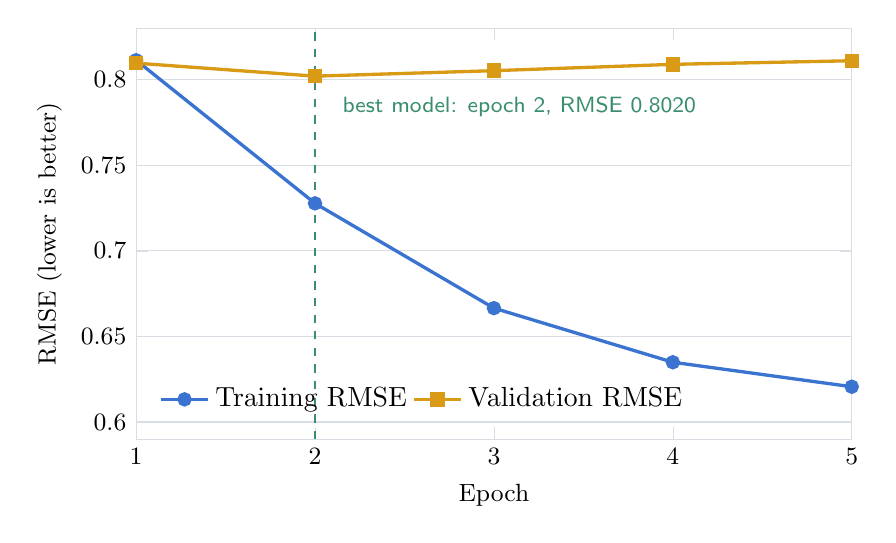
\begin{tikzpicture}
\begin{axis}[
  width=0.88\textwidth,height=68mm,
  xlabel={Epoch},ylabel={RMSE (lower is better)},
  xmin=1,xmax=5,xtick={1,2,3,4,5},
  ymin=0.59,ymax=0.83,
  ymajorgrids,grid style={draw=Rule},
  axis line style={draw=Rule},tick style={draw=Rule},
  legend style={draw=none,fill=none,at={(0.02,0.04)},anchor=south west,legend columns=2},
  label style={font=\small},tick label style={font=\small}
]
\addplot[Blue,very thick,mark=*] coordinates {
  (1,0.8113) (2,0.7277) (3,0.6665) (4,0.6349) (5,0.6206)
};
\addlegendentry{Training RMSE}
\addplot[Gold,very thick,mark=square*] coordinates {
  (1,0.8096) (2,0.8020) (3,0.8052) (4,0.8089) (5,0.8110)
};
\addlegendentry{Validation RMSE}
\addplot[Green,dashed,thick] coordinates {(2,0.59) (2,0.83)};
\node[anchor=west,font=\footnotesize\sffamily,text=Green] at (axis cs:2.10,0.784) {best model: epoch 2, RMSE 0.8020};
\end{axis}
\end{tikzpicture}
\caption{MF training and validation curves.}
\label{fig:mfcurve}
\sourceNote{Epochs 1-5 recorded in the training notebook.}
\end{figure}

Training error decreases continuously, while validation error begins to rise after epoch 2. This divergence is an early sign of overfitting. The epoch-2 weights were retained, and training stopped after epoch 5.

% -----------------------------------------------------------------------------
\section{Model 2: Implicit-Feedback ALS}
\label{sec:als}

\subsection{Converting explicit ratings into implicit preferences}

For ALS, training ratings of 4.0 or higher were treated as positive interactions. This produced 12,979,522 positive examples, representing 50.7\% of all training ratings. A total of 200,588 users had at least one positive interaction.

Each positive cell received a confidence weight of $\alpha=40$. The model was trained with the weighted least-squares formulation for implicit feedback \cite{hu2008implicit}:

\begin{equation}
\min_{\mathbf x,\mathbf y}
\sum_{u,i} c_{ui}\left(p_{ui}-\mathbf x_u^\top\mathbf y_i\right)^2
+ \lambda\left(\sum_u\|\mathbf x_u\|_2^2+\sum_i\|\mathbf y_i\|_2^2\right),
\end{equation}

where $p_{ui}$ represents the observed preference, $c_{ui}$ its confidence, and $\mathbf x_u$ and $\mathbf y_i$ the user and item factors. Alternating Least Squares alternates between regularized closed-form updates for user factors with movie factors fixed and movie factors with user factors fixed.

\subsection{Training configuration and artifact}

\begin{table}[H]
\centering
\caption{ALS-128 training configuration.}
\label{tab:alsconfig}
\begin{tabularx}{0.82\textwidth}{@{}Y r@{}}
\toprule
\textbf{Setting} & \textbf{Value} \\
\midrule
Latent factors & 128 \\
Iterations & 20 \\
Regularization & 0.05 \\
Positive-interaction threshold & $r_{ui}\geq4.0$ \\
Confidence weight $\alpha$ & 40.0 \\
Positive training interactions & 12,979,522 \\
Random seed & 0 \\
Threads & All available cores \\
Recorded training time & 3 minutes 40 seconds \\
\bottomrule
\end{tabularx}
\end{table}

The deployed artifact stores a $43{,}884 \times 128$ movie-factor matrix. Full MovieLens user factors are not required for new-user fold-in, so they were replaced by a $1 \times 128$ placeholder before saving. This keeps the ALS artifact at approximately 21.4 MiB, compared with approximately 120.5 MiB for the MF artifact containing all trained user and movie embeddings.

% -----------------------------------------------------------------------------
\section{Experimental Results and Comparison}
\label{sec:results}

\subsection{Rating prediction}

\begin{table}[H]
\centering
\caption{Rating-prediction results. Lower is better.}
\label{tab:ratingresults}
\begin{tabular}{@{}lrrrr@{}}
\toprule
\multirow{2}{*}{\textbf{Model}} & \multicolumn{2}{c}{\textbf{Validation}} & \multicolumn{2}{c}{\textbf{Test}} \\
\cmidrule(lr){2-3}\cmidrule(l){4-5}
& \textbf{RMSE} & \textbf{MAE} & \textbf{RMSE} & \textbf{MAE} \\
\midrule
Global mean & 1.0573 & 0.8272 & 1.0571 & 0.8267 \\
User + item bias & 0.8633 & 0.6537 & 0.8763 & 0.6631 \\
\textbf{MF-128} & \textbf{0.8020} & \textbf{0.5998} & \textbf{0.8244} & \textbf{0.6159} \\
\bottomrule
\end{tabular}
\sourceNote{Sections 3.1, 3.2, and 4.4 of \file{train/ml-32m-train.ipynb}.}
\end{table}

\begin{figure}[H]
\centering
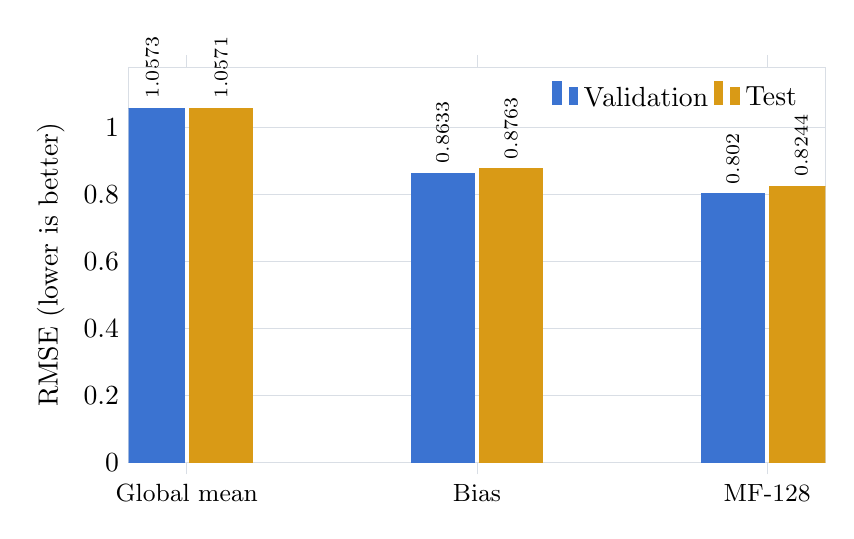
\begin{tikzpicture}
\begin{axis}[
  ybar,bar width=8mm,
  width=0.86\textwidth,height=66mm,
  ylabel={RMSE (lower is better)},ymin=0,ymax=1.18,
  symbolic x coords={Global mean,Bias,MF-128},xtick=data,
  x tick label style={align=center,font=\small},
  ymajorgrids,grid style={draw=Rule},
  axis line style={draw=Rule},tick style={draw=Rule},
  legend style={draw=none,fill=none,at={(0.98,0.98)},anchor=north east,legend columns=2},
  nodes near coords,nodes near coords style={font=\scriptsize,rotate=90,anchor=west,/pgf/number format/fixed,/pgf/number format/precision=4}
]
\addplot[fill=Blue,draw=Blue] coordinates {(Global mean,1.0573) (Bias,0.8633) (MF-128,0.8020)};
\addlegendentry{Validation}
\addplot[fill=Gold,draw=Gold] coordinates {(Global mean,1.0571) (Bias,0.8763) (MF-128,0.8244)};
\addlegendentry{Test}
\end{axis}
\end{tikzpicture}
\caption{RMSE comparison for rating prediction.}
\label{fig:rmse}
\end{figure}

MF-128 reduces test RMSE by 5.9\% and test MAE by 7.1\% relative to the bias baseline. The gain over the global mean is larger. Test RMSE is 0.0224 higher than validation RMSE, which is consistent with a more difficult chronological test period.

\subsection{Top-10 ranking}

\begin{table}[H]
\centering
\caption{Top-10 ranking results for 10,000 users. Higher is better.}
\label{tab:rankingresults}
\begin{tabular}{@{}lrrr@{}}
\toprule
\textbf{Method} & \textbf{Recall@10} & \textbf{NDCG@10} & \textbf{Evaluated users} \\
\midrule
Popularity baseline & 0.0489 & 0.0430 & 10,000 \\
Direct MF-128 ranking & 0.0005 & 0.0005 & 10,000 \\
\textbf{ALS-128} & \textbf{0.0842} & \textbf{0.0668} & 10,000 \\
\bottomrule
\end{tabular}
\sourceNote{Table values are rounded to four decimals; relative changes use the full-precision notebook outputs.}
\end{table}

\begin{figure}[H]
\centering
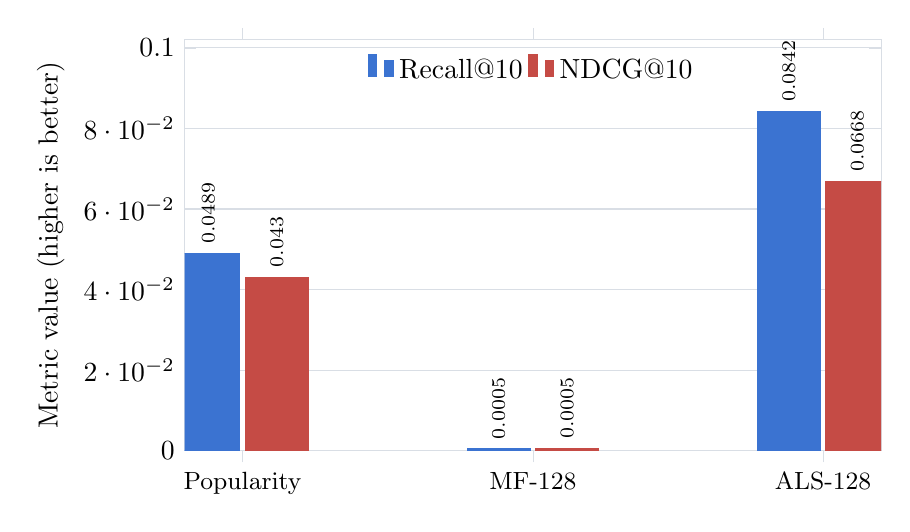
\begin{tikzpicture}
\begin{axis}[
  ybar,bar width=8mm,
  width=0.86\textwidth,height=68mm,
  ylabel={Metric value (higher is better)},ymin=0,ymax=0.102,
  symbolic x coords={Popularity,MF-128,ALS-128},xtick=data,
  x tick label style={font=\small},
  ymajorgrids,grid style={draw=Rule},
  axis line style={draw=Rule},tick style={draw=Rule},
  legend style={draw=none,fill=none,at={(0.5,0.98)},anchor=north,legend columns=2},
  nodes near coords,nodes near coords style={font=\scriptsize,rotate=90,anchor=west,/pgf/number format/fixed,/pgf/number format/precision=4}
]
\addplot[fill=Blue,draw=Blue] coordinates {(Popularity,0.0488986412) (MF-128,0.0004544802) (ALS-128,0.0841867444)};
\addlegendentry{Recall@10}
\addplot[fill=Red,draw=Red] coordinates {(Popularity,0.0430270650) (MF-128,0.0004895495) (ALS-128,0.0668026971)};
\addlegendentry{NDCG@10}
\end{axis}
\end{tikzpicture}
\caption{Top-10 ranking quality.}
\label{fig:ranking}
\end{figure}

ALS improves Recall@10 by 72.2\% and NDCG@10 by 55.3\% relative to the popularity baseline. The gains show that personalized retrieval is substantially better than recommending the same popular films to every user.

Direct MF ranking is poor: its Recall@10 is about one 185th of the ALS result. The notebook's qualitative diagnosis shows that the top MF results frequently contain films with only a few or a few dozen training ratings. Large dot products from weakly supported movie factors disrupt full-catalog ranking despite good average rating-prediction accuracy. This result supports using MF for score prediction and ALS for candidate generation.

\subsection{Task-specific model selection}

\begin{table}[H]
\centering
\caption{Experimental rationale for the model assignment.}
\begin{tabularx}{\textwidth}{@{}p{28mm}YY@{}}
\toprule
\textbf{Task} & \textbf{Selected model} & \textbf{Rationale} \\
\midrule
Candidate ranking & ALS-128 & Best Recall@10 and NDCG@10; strong personalization gain over popularity \\
Rating prediction & MF-128 & Best validation and test RMSE/MAE; direct estimates on the 0.5-5.0 scale \\
Full-catalog MF ranking & Not used & Extreme scores on rare films and very low Top-10 metrics \\
\bottomrule
\end{tabularx}
\end{table}

% -----------------------------------------------------------------------------
\section{New-User Adaptation and Production Flow}
\label{sec:serving}

The trained user factors do not include a person who uploads an IMDb or Letterboxd file after deployment. The runtime solves a new representation against the fixed movie factors without retraining either model.

\subsection{Closed-form MF fold-in}

For $n$ matched ratings, the system first estimates a damped user bias:

\begin{equation}
b_u = \frac{\sum_{i\in I_u}(r_{ui}-\mu-b_i)}{n+10}.
\end{equation}

It then uses the observed movie-factor matrix $Q_u$ and residual target $\mathbf y$ to solve the new user factor:

\begin{equation}
\mathbf p_u = \left(Q_u^\top Q_u+\lambda_u I\right)^{-1}Q_u^\top\mathbf y,
\qquad \lambda_u=\max(1,,0.02n).
\end{equation}

The factor produces predictions for all films, clipped to 0.5-5.0. The interface rounds the Letterboxd view to half-star increments and converts the same prediction to a 10-point IMDb-style display.

\subsection{ALS user recalculation}

If the training-time 4.0 like threshold does not produce enough positive examples for a new user, the runtime relaxes the threshold to 3.5 and then 3.0, seeking at least five liked films. The liked films form a one-row sparse matrix with confidence 40. The \file{implicit} library's \file{recalculate_user=True} option solves a user factor while keeping the trained movie factors fixed. All films already rated by the user are excluded from recommendations.

\subsection{Hybrid reranking}

ALS generates a pool larger than the requested recommendation list. Under the standard configuration, the pool is at least 500 films, at most 4,000, and approximately 40 times the requested list length. The final score combines the components in Table~\ref{tab:rerank}.

\begin{table}[H]
\centering
\caption{Single-user reranking components.}
\label{tab:rerank}
\begin{tabularx}{0.78\textwidth}{@{}Y r@{}}
\toprule
\textbf{Component} & \textbf{Weight} \\
\midrule
ALS candidate score & +0.50 \\
MF personalized rating prediction & +0.22 \\
Genre preference & +0.10 \\
IMDb quality and vote confidence & +0.08 \\
Similarity to liked films & +0.08 \\
Novelty & +0.02 \\
Similarity to disliked films & $-0.16$ \\
\bottomrule
\end{tabularx}
\end{table}

A diversity penalty similar to maximal marginal relevance reduces near-duplicate recommendations in the final list. The ``because you liked'' explanations use cosine similarity between normalized ALS movie factors.

\begin{figure}[H]
\centering
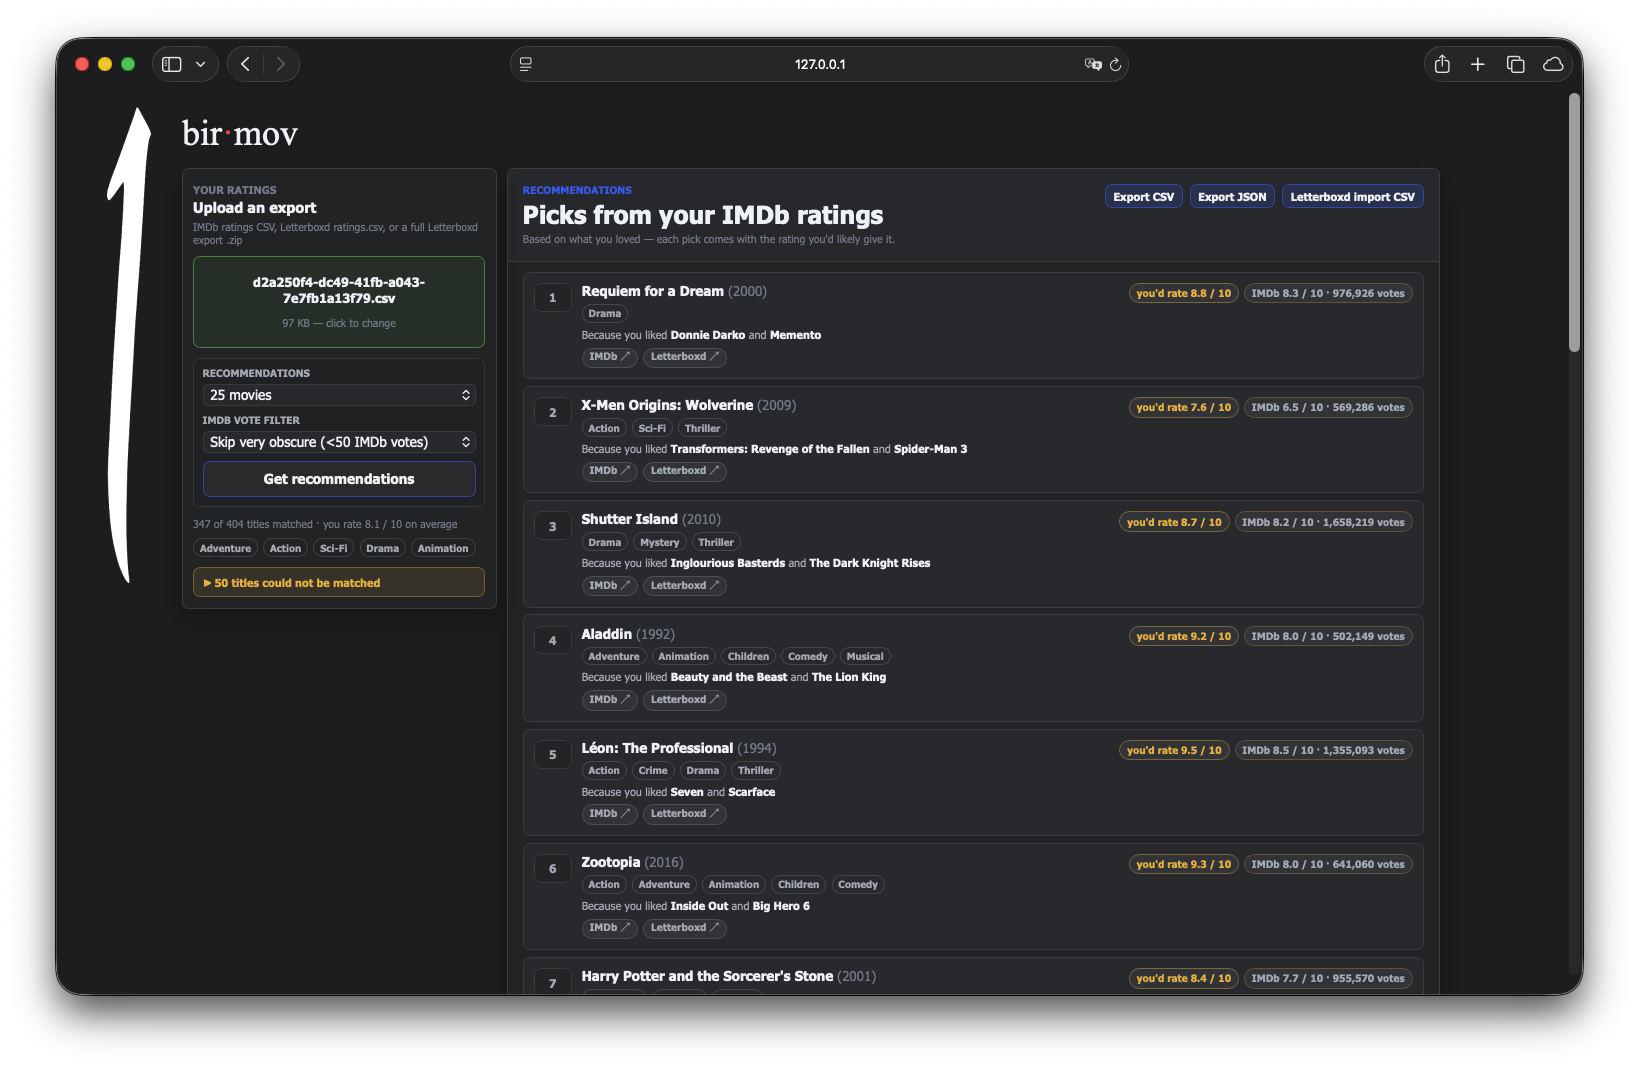
\includegraphics[width=0.94\textwidth]{screenshot.png}
\caption{The bir.mov interface using both models. The gold badge reflects the MF rating prediction, while the recommendation order reflects the hybrid ranking.}
\label{fig:ui}
\sourceNote{Project file \file{docs/screenshot.png}.}
\end{figure}

% -----------------------------------------------------------------------------
\section{Limitations and Threats to Validity}

\begin{itemize}
  \item \textbf{Single random seed:} MF and ALS use seed 0, and ranking evaluation also samples users with seed 0. Multiple runs and confidence intervals were not reported, so sensitivity to randomness remains unmeasured.
  \item \textbf{Hyperparameter search:} The notebook does not record a systematic grid search, Bayesian optimization, or cross-validation study. The selected settings are a valid operating point, but are not proven globally optimal.
  \item \textbf{Information loss in ALS:} Ratings of 4.0 and 5.0 become the same positive signal. Rating magnitude and low-rating negative evidence are not used by the base ALS training objective.
  \item \textbf{Ranking candidate set:} Test evaluation excludes training items, but validation items are not separately removed. Alternative candidate definitions can change the absolute metric levels.
  \item \textbf{Long-tail tradeoff:} The minimum-5-ratings filter reduces noise but removes new and highly niche films from the vocabulary. Production IMDb vote filters also influence the balance between discovery and confidence.
  \item \textbf{Hybrid-layer evaluation:} The reranking weights are defined in production code, but the combined list has not been separately measured for Recall/NDCG, diversity, novelty, and user satisfaction in this experiment.
  \item \textbf{Temporal and community bias:} MovieLens represents interactions from 1995-2023 and its own user community. Generalization to current releases, countries, languages, and demographic groups requires separate validation.
  \item \textbf{No online measurement:} Offline gains do not guarantee higher click, watch, or satisfaction rates. No A/B test or shadow-traffic evaluation has been recorded.
\end{itemize}

These limitations do not invalidate the task assignment between the models; they identify the most important directions for further evaluation.

% -----------------------------------------------------------------------------
\section{Conclusion and Recommended Next Steps}

The experiments reveal two clearly different strengths. MF-128 is the best rating predictor, with test RMSE 0.8244 and MAE 0.6159. ALS-128 is clearly superior for Top-10 retrieval, achieving Recall@10 of 0.0842 and NDCG@10 of 0.0668, respectively 72.2\% and 55.3\% above the popularity baseline. MF's failure as a full-catalog ranker demonstrates that low RMSE alone does not imply a useful recommendation list.

The current assignment is therefore technically justified: \textbf{ALS finds candidates; MF predicts ratings}. Runtime fold-in adapts both models to a new user without full retraining, while the hybrid layer adds quality, genre, similarity, negative-preference, and diversity signals.

The recommended sequence of follow-up experiments is:

\begin{enumerate}
  \item Compare the hybrid reranker with pure ALS under the same chronological protocol using Recall@10, NDCG@10, catalog coverage, novelty, and intra-list diversity.
  \item Learn reranking weights on validation data instead of fixing them manually, and evaluate group-recommendation weights separately.
  \item Run multi-seed searches over ALS confidence, regularization, factor count, and like threshold, as well as MF factor count and L2 strength.
  \item Investigate the rare-film score explosions in direct MF ranking with minimum-support constraints, factor-norm clipping, and ranking objectives such as BPR.
  \item Evaluate fold-in quality by user-history length, particularly for 1-4, 5-19, and 20+ matched ratings.
  \item Validate offline gains against real user behavior through a privacy-preserving online experiment.
\end{enumerate}

% -----------------------------------------------------------------------------
\appendix
\section{Reproducibility and Source Traceability}

\subsection{Recorded training environment}

\begin{table}[H]
\centering
\caption{Training environment recorded in the notebook.}
\begin{tabularx}{0.82\textwidth}{@{}Y r@{}}
\toprule
\textbf{Component} & \textbf{Version / value} \\
\midrule
Python & 3.14.6 \\
Platform & macOS 26.5.1, arm64 \\
NumPy & 2.5.0 \\
pandas & 3.0.3 \\
SciPy & 1.18.0 \\
Matplotlib & 3.11.0 \\
PyTorch & 2.12.1 \\
implicit & 0.7.3 \\
CUDA / MPS & No / Yes \\
Selected device & MPS \\
PyTorch threads & 4 \\
\bottomrule
\end{tabularx}
\end{table}

\subsection{Source-file mapping}

{\small
\begin{tabularx}{\textwidth}{@{}p{57mm}Y@{}}
\toprule
\textbf{File} & \textbf{Role in this report} \\
\midrule
\file{train/ml-32m-train.ipynb} & Data analysis, filtering, chronological split, baselines, MF and ALS training, and recorded metrics \\
\file{model/ml32m-mf128-v1/meta.json} & MF artifact name, dimensions, factor count, and exact best validation RMSE \\
\file{model/ml32m-als128-v1/meta.json} & ALS iterations, regularization, confidence, positive-example count, and artifact scope \\
\file{app/recommender.py} & New-user fold-in equations, candidate generation, and hybrid reranking weights \\
\file{README.md} & Project purpose, model roles, and deployment overview \\
\bottomrule
\end{tabularx}
}

The model artifacts carry a saved-at timestamp of July 2, 2026 UTC. This report was prepared on July 17, 2026 by reading the files above. Because the raw MovieLens files and training pipeline were not rerun, the values presented here are a traceable technical summary of the recorded experiment rather than a new execution.

\begin{thebibliography}{9}

\bibitem{harper2015movielens}
F. M. Harper and J. A. Konstan,
\enquote{The MovieLens Datasets: History and Context},
\textit{ACM Transactions on Interactive Intelligent Systems}, vol. 5, no. 4, 2015.
\href{https://doi.org/10.1145/2827872}{doi:10.1145/2827872}.

\bibitem{koren2009mf}
Y. Koren, R. Bell, and C. Volinsky,
\enquote{Matrix Factorization Techniques for Recommender Systems},
\textit{Computer}, vol. 42, no. 8, pp. 30-37, 2009.
\href{https://doi.org/10.1109/MC.2009.263}{doi:10.1109/MC.2009.263}.

\bibitem{hu2008implicit}
Y. Hu, Y. Koren, and C. Volinsky,
\enquote{Collaborative Filtering for Implicit Feedback Datasets},
\textit{2008 Eighth IEEE International Conference on Data Mining}, pp. 263-272, 2008.
\href{https://doi.org/10.1109/ICDM.2008.22}{doi:10.1109/ICDM.2008.22}.

\bibitem{movielens32m}
GroupLens Research,
\enquote{MovieLens 32M Dataset}.
\url{https://grouplens.org/datasets/movielens/32m/}.

\bibitem{birMovNotebook}
bir.mov Project,
\enquote{MovieLens ml-32m Recommendation Model Pipeline},
\file{train/ml-32m-train.ipynb}, recorded notebook in the project workspace.

\end{thebibliography}

\end{document}
